\documentclass[sigconf]{acmart}

\usepackage{booktabs} % For formal tables
\usepackage{CJK}
\usepackage{ctex}
\usepackage{color}
\usepackage{graphicx}
\usepackage{amssymb}
\usepackage{amsmath}
\usepackage{amsthm}
\usepackage{booktabs}


\usepackage{fancyhdr}
\usepackage{extramarks}
\usepackage{amsfonts}
\usepackage{tikz}
\usepackage[plain]{algorithm}
\usepackage{algpseudocode}
\usepackage{listings}

% Copyright
\setcopyright{none}

%Conference
\acmConference{Data Communication}{May 2018}{Nanjing, China} 
%\acmYear{2018}
%\copyrightyear{2018}

%\acmPrice{15.00}


\begin{document}
\begin{CJK}{UTF8}{song}

\title{降低移动网页浏览器能耗的技术综述}
%\titlenote{Produces the permission block, and copyright information}
%\subtitle{Extended Abstract}

\author{徐子恒 161160037, 赖伟 161250052}
%\authornote{Note}$  $
\orcid{1234-5678-9012}
\affiliation{%
  \institution{计算机科学与技术系}
}
\email{161160037@smail.nju.edu.cn,  161250052@smail.nju.edu.cn}

% The default list of authors is too long for headers}
%\renewcommand{\shortauthors}{F. Lastname et al.}


\begin{abstract}

智能手机已经成为了人们生活中必不可少的电子移动设备,但是应用的高能耗导致智能手机的续航始终是一个难以克服的挑战。网页浏览器是智能手机中最核心的应用之一。但因为移动浏览器在性能上进行了大量优化,给移动设备的能源带来了巨大的负担。因此,我们所要介绍的技术正是为了减少智能手机加载网页所消耗的能源,同时尽可能不增加页面加载时间和损害用户体验。

\end{abstract}

%
% The code below should be generated by the tool at
% http://dl.acm.org/ccs.cfm
% Please copy and paste the code instead of the example below. 
%
\begin{CCSXML}
<ccs2012>
 <concept>
  <concept_id>10010520.10010553.10010562</concept_id>
  <concept_desc>Computer systems organization~Embedded systems</concept_desc>
  <concept_significance>500</concept_significance>
 </concept>
 <concept>
  <concept_id>10010520.10010575.10010755</concept_id>
  <concept_desc>Computer systems organization~Redundancy</concept_desc>
  <concept_significance>300</concept_significance>
 </concept>
 <concept>
  <concept_id>10010520.10010553.10010554</concept_id>
  <concept_desc>Computer systems organization~Robotics</concept_desc>
  <concept_significance>100</concept_significance>
 </concept>
 <concept>
  <concept_id>10003033.10003083.10003095</concept_id>
  <concept_desc>Networks~Network reliability</concept_desc>
  <concept_significance>100</concept_significance>
 </concept>
</ccs2012>  
\end{CCSXML}

%\ccsdesc[500]{Computer systems organization~Embedded systems}
%\ccsdesc[300]{Computer systems organization~Redundancy}
%\ccsdesc{Computer systems organization~Robotics}
%\ccsdesc[100]{Networks~Network reliability}

% We no longer use \terms command
%\terms{Theory}

\keywords{智能手机; 移动网络浏览器; 网页加载; 能源效率}


\maketitle

\section{Introduction}

网页浏览器是智能手机中最核心的应用之一。但因为移动浏览器在性能上进行了大量优化,给移动设备的能源带来了巨大的负担。因此我们希望提高网页浏览的能效,特别是减少网页加载的能耗。 本文中介绍的技术试图在不影响用户体验且不增加页面加载时间的情况下降低智能手机上网页加载的能耗。

首先,我们会介绍浏览器内部的体系结构和系统行为,以了解能量是如何被用于加载网页,从而发现提高能效的机会。尽管许多浏览器制造商都在努力提高移动设备的能效,但先前的调查结果表明,目前的移动浏览器尚未完全针对网页加载进行能源优化。 首先,不管网络条件如何,网络资源处理总是在积极进行,这就带来了能源效率低下的风险。 其次,渲染率过高,导致大量能量被消耗而没有带来用户可感知的好处。最后,拥有新兴的ARM big.LITTLE架构[3]的现代CPU的节电能力未得到充分利用。 从根本上说,在网页加载过程中过度优化了性能表现,而忽视了能源成本。

为了降低网页加载的能耗,必须重新考虑能源性能的权衡,以制定网页加载的新设计原则。本文会介绍基于这些原则的三种新技术,每种技术对应解决了上述能效问题之一。第一种是使用$network-aware\ resource\ processing$(NRP)技术来适应不断变化的网络条件,从而实现能耗的降低。这种技术使用了自适应资源缓冲技术来动态控制资源下载速度,从而在不增加页面加载时间的情况下提高能源效率。第二种技术是$adaptive\ content\ painting$(ACP)技术,这种技术可以避免不必要的内容渲染,从而达到减少能源开销的目的。并在节能和页面加载时间之间做出权衡来确保用户体验不会受到影响。最后,为了更好地利用big.LITTLE架构,可以使用$application-assisted\ scheduling$(AAS)技术来利用浏览器的内部知识来制定更好的调度决策。具体来说,这种技术采用了基于QoS反馈的自适应线程调度,只要满足相关QoS要求,浏览器就可以让线程在小内核上运行以节约能源。

我们通过修改Chromium浏览器在商业智能手机上实施了所有这三项技术。总体而言,这些技术大大降低了网页加载的能源成本。使用美国Alexa排名前100的网站进行的实验评估表明,在使用WiFi的big.LITTLE智能手机上,我们修订后的Chromium浏览器能够实现平均24.4%的系统节能,同时减少0.38%的页面加载时间,而默认的Chromium浏览器。在使用3G时,平均系统节能为22.5%,平均页面加载时间为0.41%。在另一款没有big.LITTLE支持的智能手机上,我们的技术在使用WiFi时平均可以减少11.7%的能耗。我们还进行了用户研究,以确认我们的技术不会影响用户的感知体验。此外,所有参与者都表明他们的意图(或兴趣)总是使用我们的技术(72%)或电池电量不足(28%)。

尽管我们的实施基于Chromium,但我们提出的技术也可以应用于其他移动浏览器。 Chromium的前两个能源效率问题与Web内容下载,处理和绘画的一般程序有关。 因此,其他移动浏览器通常会遇到相同的问题,但具有不同的重要级别。 除Chromium之外,我们还将Firefox的ACP和AAS技术应用到Firefox,即使没有对Firefox内部的深入了解,也导致平均节省大量的能源(10.5%),页面加载时间略微增加(1.69%) ,与默认的Firefox相比。


\section{Background} 

在本节中,我们将介绍Chromium浏览器和big.LITTLE体系结构。

\subsection{Chromium Browser Architecture}

\begin{figure}[htbp]
	\centering
	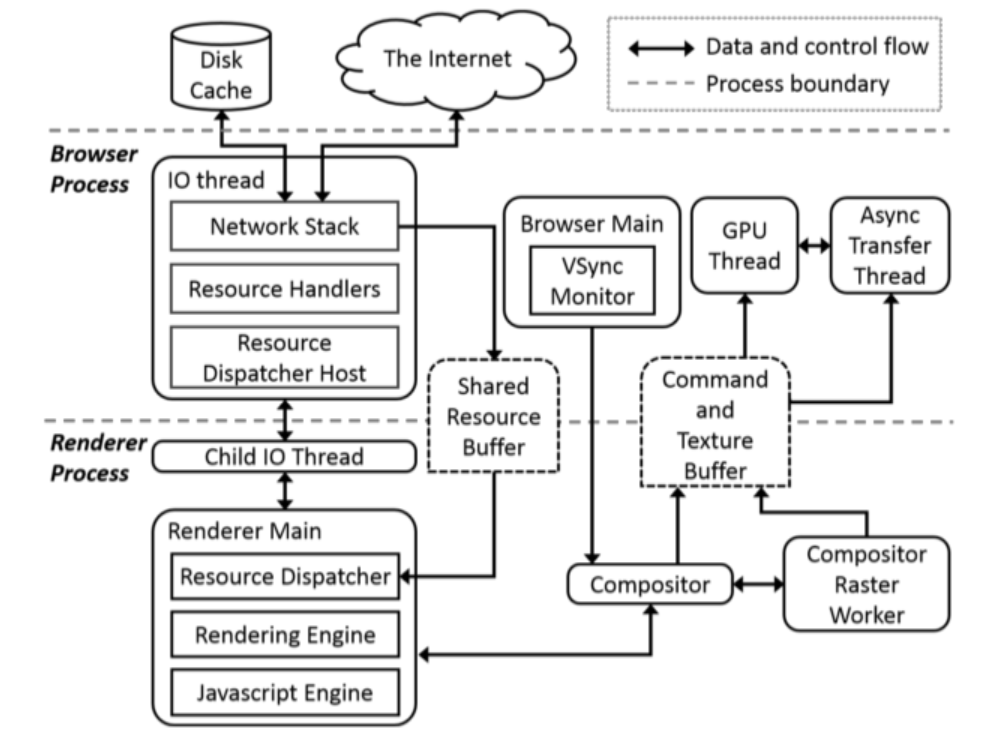
\includegraphics[width=3.4in]{./figure/figure1}
	\caption{Chromium浏览器的体系结构}\label{fig:tasks}
\end{figure}

如图1所示, Chromium使用单个浏览器进程和多个Renderer进程的多进程体系结构。 每个Renderer进程运行渲染引擎的实例(以前是WebKit [14],现在是Blink [4])以及解析和执行Web内容的JavaScript引擎。 每个Renderer进程通常对应于Web浏览器UI中的一个选项卡。 浏览器进程运行网络堆栈并从网络中为所有呈现器进程获取网络资源,从而在所有呈现器进程之间共享高效的网络资源。 渲染器进程在沙盒环境中运行,对客户端设备和网络的访问受限,防止渲染引擎中的漏洞侵害整个Web浏览器。

\section{Problem}
问题描述

\section{Overview}
已有工作分类,介绍

\subsection{class 1}
有一些工作从用户的角度 ...



方法结构图,如图 \ref{fig:tasks} 


\subsection{class 2}
还有一些工作从环境的角度 ...

\section{conclusion}
结论

注意:参考文献必须完整


\bibliographystyle{ACM-Reference-Format}
\bibliography{sigproc} 

\end{CJK}{UTF8}{song}
\end{document}
